\documentclass{article}
\title{Nechyba Ch.10 消费者剩余与无谓损失}
\author{Dawei Wang}
\date{\today}
\usepackage{ctex}
\usepackage{amsmath}
\usepackage{amssymb}
\usepackage{graphicx} %插入图片的宏包
\usepackage{float} %设置图片浮动位置的宏包
\usepackage{subfigure} %插入多图时用子图显示的宏包
\begin{document}
	\maketitle
通过向消费者询问为了避免某种特殊的情况发生他们愿意付出多少钱,或者说当情况发生改变时他们需要多少经济上的补偿,我们就可以找到方法量化在不同经济情况下消费者福利变化了多少。

如果某项政策的受益者所获利益多于利益受损者所损失的利益,那么原则上与这项政策伴随的将会是一个补偿机制,这个补偿机制会使得这项政策一致通过。

\section{A 以美元度量消费者福利}

消费者剩余:消费者愿意花多少钱进入市场。

边际支付意愿:假如已经选择了最优点A,那么我愿意为获得这一加仑汽油($ x_1 $)支付多少,即对于开始的第一加仑汽油,可以通过求出无差异曲线在1加仑处的斜率(MRS)来计算我的支付意愿。

\hspace*{\fill}

边际支付意愿曲线又被称作补偿需求曲线,常规的需求曲线被称为非补偿需求曲线。只有当偏好是拟线性时,补偿需求曲线才和非补偿需求曲线重合。

补偿需求曲线只包括替代效应而非补偿需求曲线则包括替代效应和收入效应。

因为只包括替代效应,MWTP一定是向下倾斜的。

\hspace*{\fill}

总支付意愿与消费者剩余:首先确定在市场上购买汽油($ x_1 $)的总支付意愿。其次,在这个数量基础上减去我实际在市场需要支付的价格。二者的差就是我能够进入这个市场给我带来的福利——即我愿意支付的价格比我实际支付的价格多多少。

消费者剩余:我愿意为我消费的汽油所支付的数量减去我实际上支付的数量所得的结果,就是我们表示出来的两个面积的插值。这就是我能够进入这个市场给我带来的福利,即我为进入价格为P的汽油市场所愿意支付的最大数量。

\hspace*{\fill}

如果被征税的人愿意贿赂政府的最大数目比他实际缴纳的税还多,从而可以得知,至少从理论上,政府可以通过某种方法从这个人身上获取更多的收入而不使他的福利变差。假设的贿赂数目与实际缴纳数目之间的差就是政府在不使个体福利变差的情况下所能增加的收入,这就是无谓损失(DWL)。

考虑替代性很强的两种商品$ x_1 $和$ x_2 $,若政府对$ x_1 $征税,则消费者不消费$ x_1 $转而去消费$ x_2 $,结果是政府即未实际征收到对$ x_1 $的税,消费者的福利还下降了,这种下降就叫做无谓损失。

税收通过调整经济中的相对价格使消费者、工人和储蓄者从征税的商品和服务转向不征税的商品和服务。只要有机会成本变化,这种替代活动就会发生,且税收会增加替代效应,从这些角度来看,税收作为增加收入的手段是扭曲且无效率的。

无谓损失都是由替代效应造成的。
\begin{figure}[H] %H为当前位置,!htb为忽略美学标准,htbp为浮动图形
	\centering %图片居中
	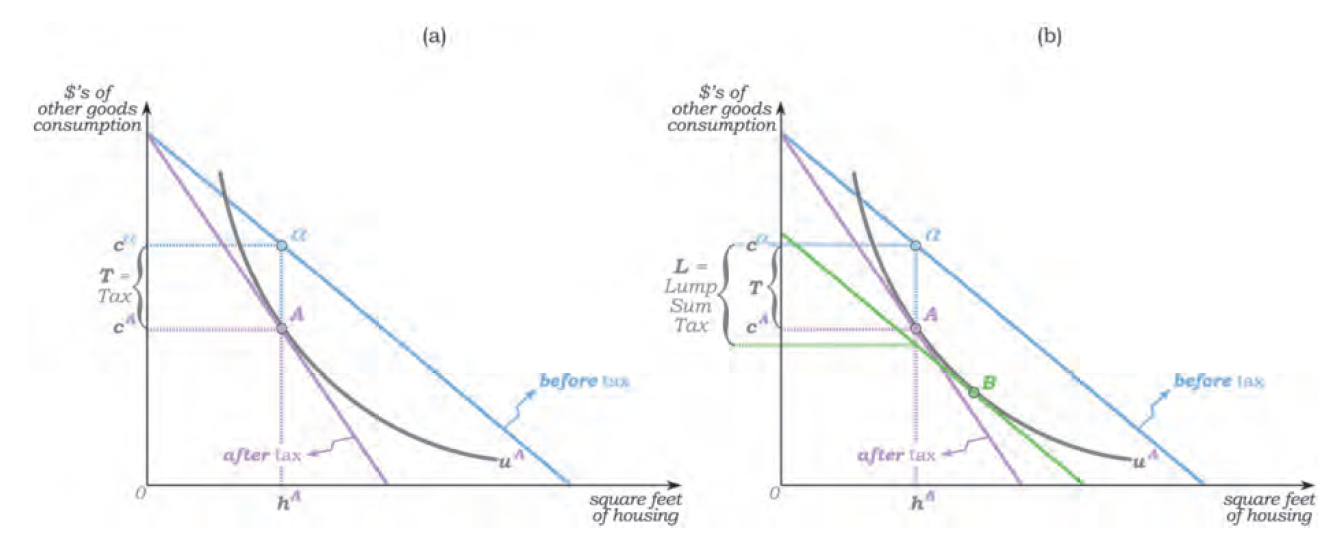
\includegraphics[width=1\textwidth]{DWL} %插入图片,[]中设置图片大小,{}中是图片文件名
	\caption{Deadweight Losses and Substitution Effect} %最终文档中希望显示的图片标题
	\label{Fig.main2} %用于文内引用的标签
\end{figure}

L表示用一次性税收从这位消费者处所能征收的数额。一次性税收(lump sum tax)是一种不会改变机会成本的税收(预算线斜率)。T和L的差就是对房子征税所带来的无谓损失。从一种商品征税的角度来说,一次性税收就是一种能够在不使得他人福利减少的情况下让某些人变得更好的方法。从而可以说对单一商品征税是无效的。

\hspace*{\fill}

无谓损失与替代效应:随着替代效应消失,改变机会成本的税收所带来的无谓损失也一同消失;若偏好的替代性增强,则无谓损失也随之增强。

\begin{figure}[H] %H为当前位置,!htb为忽略美学标准,htbp为浮动图形
	\centering %图片居中
	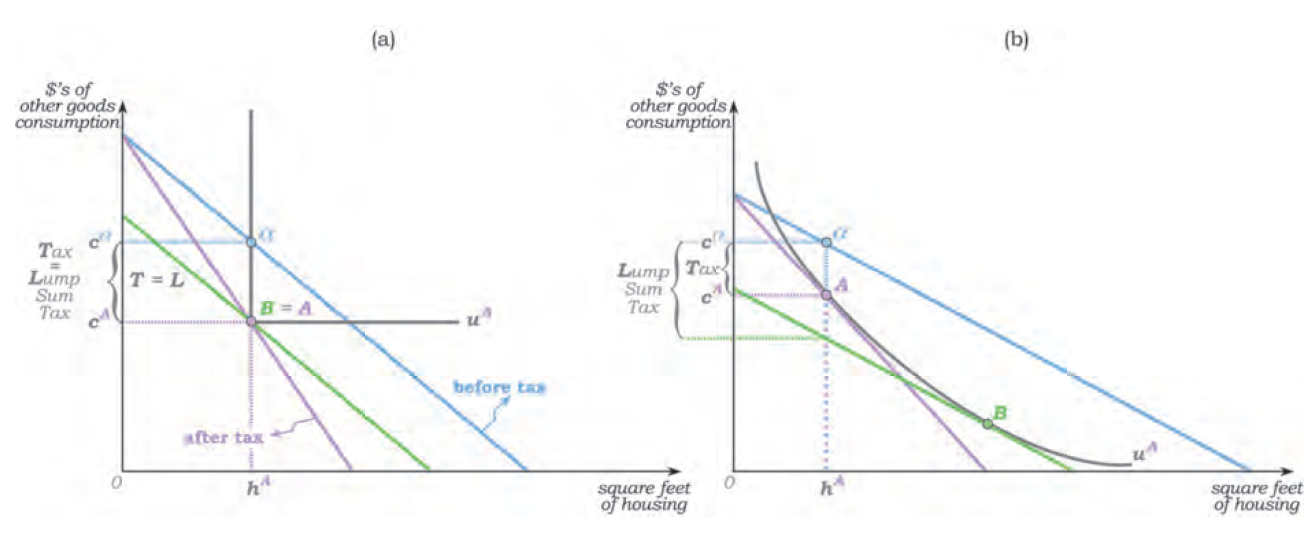
\includegraphics[width=1\textwidth]{DWL_1} %插入图片,[]中设置图片大小,{}中是图片文件名
	\caption{Distortionary Taxes and Substitution Effects} %最终文档中希望显示的图片标题
	\label{Fig.main3} %用于文内引用的标签
\end{figure}

消费者减少对征税商品的消费并不是导致税收无效率的原因。替代效应才是消费者行为改变使得税收无效率的内在原因。

无谓损失正是当税收导致机会成本改变进而带来替代效应时会发生的事情。

\hspace*{\fill}

现实中的税收几乎全是无效率的,不考虑外部性,只有两种情形下税收可能会是有效的:

1. 税收没有改变机会成本(一次性税收);

2. 即时税收改变了机会成本,但并没有引起替代效应。

考虑外部性的情况下则税收也有可能是有效的。

\hspace*{\fill}

现实中一次性税收很难实现,因为它必须使消费者不能采用任何替代行为来规避任何一点税收。

\hspace*{\fill}

度量在MWTP上的DWL:

\begin{figure}[H] %H为当前位置,!htb为忽略美学标准,htbp为浮动图形
	\centering %图片居中
	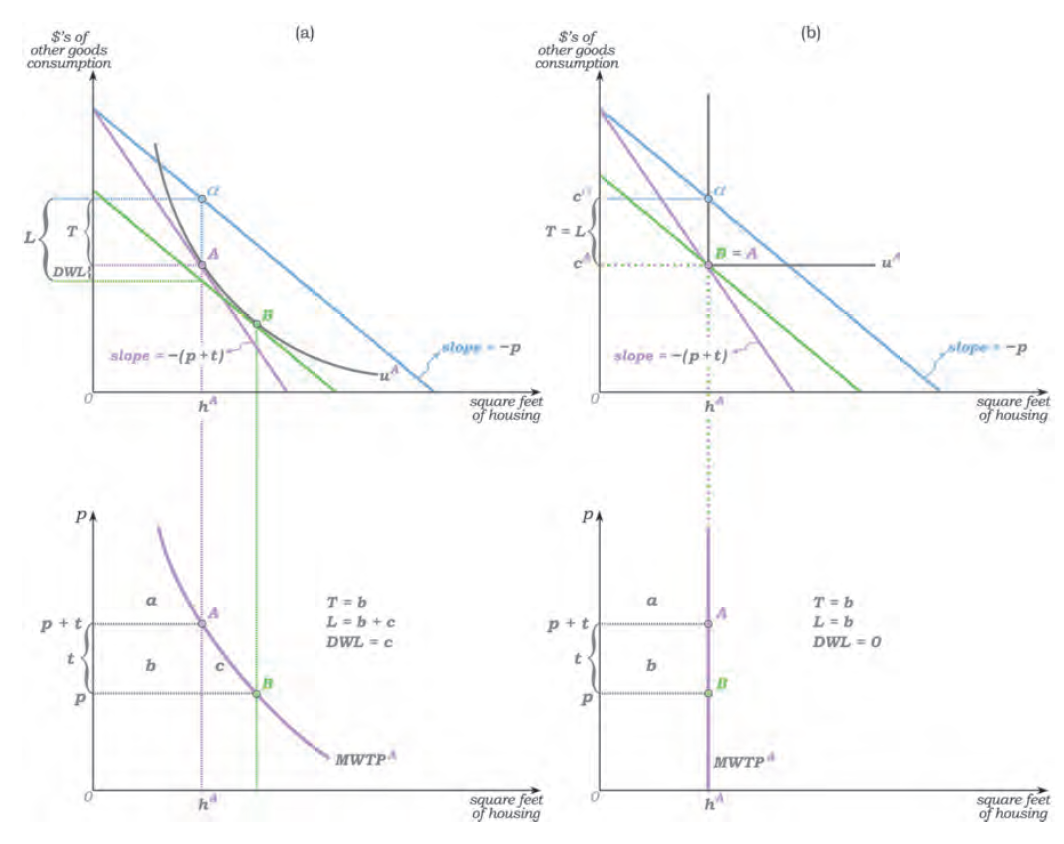
\includegraphics[width=1\textwidth]{DWL_2} %插入图片,[]中设置图片大小,{}中是图片文件名
	\caption{Translating DWL to MWTP Curves} %最终文档中希望显示的图片标题
	\label{Fig.main4} %用于文内引用的标签
\end{figure}

\hspace*{\fill}

DWL的指数型增长与大税基情况:随着某种商品的税率增加,税收带来的无谓损失将以更快的速度增长。当税率乘以x时,无谓损失将变为原来的$ x^2 $倍。

从效率的角度来说,税率更低但税基范围更广比税率较高但税基较小更合适。

\section{消费者福利的数学运算与对偶性}
\subsection{效用最大化与支出最小化的对偶}

消费者效用最大化问题:

\[
\max\limits_{x_1,x_2}u(x_1,x_2)\quad s.t.\quad p_1x_1+p_2x_2=I
\]

其解为(非补偿)需求函数:
\[
x_1=x_1(p_1,p_2,I)\qquad x_2=x_2(p_1,p_2,I)
\]

支出最小化问题:

\[
\min\limits_{x_1,x_2}E=p_1x_1+p_2x_2\quad s.t.\quad u(x_1,x_2)=u
\]

其解为补偿性需求函数:

\[
x_1=h_1(p_1,p_2,I)\qquad x_2=h_2(p_1,p_2,I)
\]

间接效用函数:任何经济情况下,当消费者做到最好时,他所能获得的效用

\[
V(p_1,p_2,I)=u(x_1(p_1,p_2,I),x_2(p_1,p_2,I))
\]

支出函数:对于任何价格和效用水平,消费者最少需要多少预算才能达到这个效用水平

\[
E(p_1,p_2,u)=p_1h_1(p_1,p_2,u)+p_2h_2(p_1,p_2,u)
\]

在需求曲线中,用支出函数代替需求函数中的收入变量I,接着不固定收入,而是构建一个新的需求函数,使得消费者总是有足够的收入来达到效用水平u,这正是补偿需求函数的准确定义。因此,可以得到如下逻辑关系:

\[
x_i(p_1,p_2,E(p_1,p_2,u))=h_i(p_1,p_2,u)
\]

\[
x_i(p_1,p_2,V(p_1,p_2,I))=x_i(p_1,p_2,I)
\]

\begin{figure}[H] %H为当前位置,!htb为忽略美学标准,htbp为浮动图形
	\centering %图片居中
	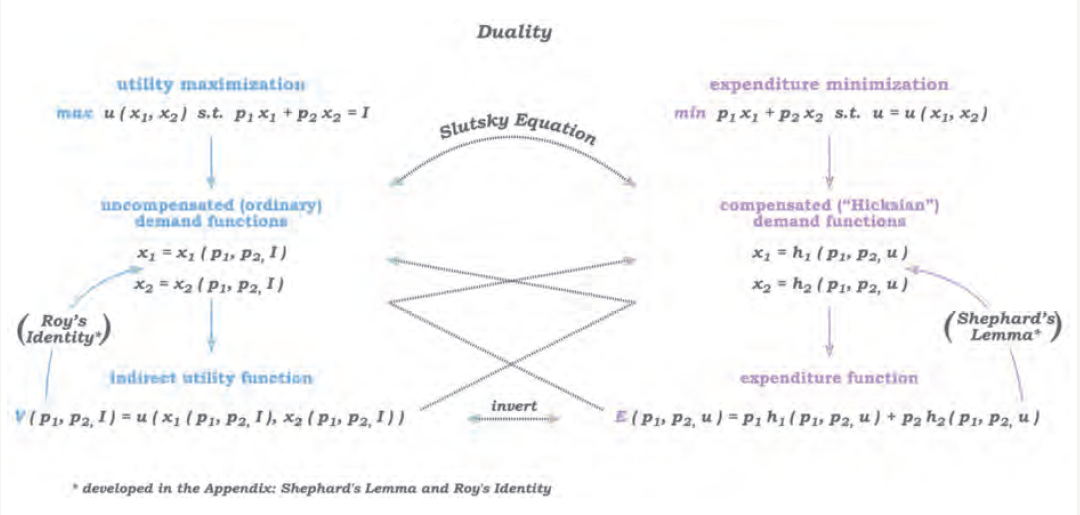
\includegraphics[width=1\textwidth]{DWL_3} %插入图片,[]中设置图片大小,{}中是图片文件名
	\caption{“Duality” of Utility Maximization and Expenditure Minimization} %最终文档中希望显示的图片标题
	\label{Fig.main5} %用于文内引用的标签
\end{figure}

\hspace*{\fill}

Slutsky function:描述非补偿需求曲线和补偿需求曲线斜率关系的方程

对
\[
x_i(p_1,p_2,E(p_1,p_2,u))=h_i(p_1,p_2,u)
\]
两侧分别求关于价格的偏导:
\[
\frac{\partial x_i}{\partial p_j}+(\frac{\partial x_i}{\partial E})(\frac{\partial E}{\partial p_j})=\frac{\partial h}{\partial p_j}
\]
改写为:
\[
\frac{\partial x_i}{\partial p_j}=\frac{\partial h}{\partial p_j}-(\frac{\partial x_i}{\partial E})(\frac{\partial E}{\partial p_j})
\]

利用对偶性概念计算无谓损失

\[
T=tx_1(p_1+t,p_2,I)
\]
\[
L=I-E(p_1,p_2,V(p_1+t,p_2,I))
\]

Shephard's Lemma:
\[
\frac{\partial E(p_1,p_2,u)}{\partial p_i}=h_i(p_1,p_2,u)
\]

Roy's Identity
\[
-\frac{\partial V(p_1,p_2,I)/\partial p_i}{\partial V(p_1,p_2,I)/\partial I}=x_i(p_1,p_2,I)
\]

\hspace*{\fill}

Shephard's Lemma背后的直觉与支出函数的凹性

替代效应意味着随着横轴上价格的改变,支出函数的切线的斜率随之改变并且支出函数是价格的凹函数,即:

\[
\frac{\partial E(p_1,p_2,u)}{\partial p_i}>0\qquad and\qquad \frac{\partial^2E(p_1,p_2,u)}{\partial p_i^2}\le 0
\]




\end{document}